\documentclass[a4paper, twoside, openany]{NCEPUDoctor}
\usepackage{multirow}
\usepackage{titlesec}
\usepackage{amssymb}
\usepackage{wasysym}
\usepackage{changepage}
\usepackage{ifthen} 
\usepackage{fancyhdr}
\usepackage{graphicx}
\usepackage{adjustbox}
\usepackage{caption}
\usepackage{xcolor}
\usepackage{booktabs}
\usepackage{microtype}
\usepackage{array,tabularx}
\captionsetup[table]{labelsep=space} 
\makeatletter
\renewcommand\bibsection{}
\makeatother
\usepackage{longtable}
%%%%%-------------------对以下内容进行编辑------------------------

    %% ============================================
    %% 设置学位类型（二选一）
    %% ============================================   
    %% ============================================
    %% 学术博士信息填写示例
    %% ============================================
    \degreetype{academic}      % 学术博士
    % 中文信息
    \ctitlezh{智能电网关键关键技术研究与应用}  % 中文标题
    \cauthorzh{张三}   % 作者姓名
    \cadvisorzh{李教授}   % 导师姓名
    \cdegreezh{工学博士}  % 申请学位
    \csubjectzh{电气工程} % 学科
    \cmajorzh{电力系统及其自动化}   % 专业
    \cschoolzh{电气与电子工程学院}  % 所在学院
    \cdatezh{2024年6月}   % 答辩日期
    
    % 英文信息
    \ctitleen{Research on Power System Fault Diagnosis Based on Deep Learning}  % 英文标题
    \Ltitle{False} % False: 英文标题过长时使用小2号字体，True: 正常使用2号字
    \cauthoren{Zhang San}  % 作者姓名
    \cadvisoren{Prof. Li}  % 导师姓名
    \ccosupervisoren{Prof. Wang}    % 联合导师（学术博士）
    \cdegreeen{Doctor of Engineering}  % 申请学位
    \csubjecten{Electrical Engineering}   % 学科
    \cmajoren{Power System and Its Automation}   % 专业
    \cschoolen{School of Electrical and Electronic Engineering}   % 所在学院
    \cdateen{June, 2024}  % 答辩日期

    % % ============================================
    % % 专业博士信息填写示例
    % % ============================================
    % \degreetype{professional}  % 先设置为专业博士
    % % 中文信息
    % \ctitlezh{智能电网关键技术研究与应用}  % 中文标题
    % \cauthorzh{王五}       % 作者姓名
    % \cadvisorzh{赵教授}    % 导师姓名
    % \cmentorzh{孙工程师}            % 企业导师（专业博士）
    % \cdegreezh{能源动力}            % 申请学位
    % \csubjectzh{电气工程}           % 专业领域
    % \cclutivationzh{全日制/非全日制}       % 学习方式
    % \cschoolzh{电气与电子工程学院}
    % \cdatezh{2024年6月}
    
    % % 英文信息
    % \ctitleen{Research and Application of Key Technologies in Smart Grid}  % 英文标题
    % \Ltitle{False} % False: 英文标题过长时使用小2号字体，True: 使用2号字，可根据标题自行设置字号
    % \cauthoren{Wang Wu}  % 作者姓名
    % \cadvisoren{Prof. Zhao}  % 导师姓名
    % \cmentoren{Engineer Sun}   % 企业导师（专业博士）
    % \cdegreeen{Doctor of Engineering}  % 申请学位
    % \csubjecten{Electrical Engineering}  % 专业
    % \cclutivationen{Full-time/Part-time}   % 学习方式
    % \cschoolen{School of Electrical and Electronic Engineering}   % 所在学院
    % \cdateen{June, 2024}  % 答辩日期

    % =====================图书分类号和密级设置=======================
    % %图书分类号
    \cclc{xxxx}
    \cudc{xxxx}
    % % 设置密级，可选值如下：
    \csecretlevel{public}      % 公开（默认）
    % \csecretlevel{internal}    % 内部
    % \csecretlevel{secret}      % 秘密
    % \csecretlevel{confidential}% 机密
    % \csecretlevel{topsecret}   % 绝密
  
  
\begin{document}
  \maketitlepage            % 封面
  \makechinainfopage        % 中文信息页
  \makeenglishinfopage      % 英文信息页
  \makestatement            % 原创性声明
  \setcounter{page}{1} % 页码重置
\pagenumbering{Roman} % 设置页码格式为罗马数字

\chapterstar[摘要]{摘\qquad 要}
\echapterstar{Abstract (In Chinese)}

\begin{abstract}{关键词1；关键词2；关键词3；关键词4；关键词5}
\sloppy  % 中文摘要分散对齐
摘要是论文内容的高度概括，应具有独立性和自含性，即不阅读论文的全文，就能获得必要的信息。摘要应包括本论文的目的、主要研究内容、研究方法、创造性成果及其理论与实际意义。摘要中不宜使用公式、化学结构式、图表和非公知公用的符号和术语，不标注引用文献编号。避免将摘要写成目录式的内容介绍。摘要是论文内容的高度概括，应具有独立性和自含性，即不阅读论文的全文，就能获得必要的信息。摘要应包括本论文的目的、主要研究内容、研究方法、创造性成果及其理论与实际意义。摘要中不宜使用公式、化学结构式、图表和非公知公用的符号和术语，不标注引用文献编号。避免将摘要写成目录式的内容介绍。摘要是论文内容的高度概括，应具有独立性和自含性，即不阅读论文的全文，就能获得必要的信息。摘要应包括本论文的目的、主要研究内容、研究方法、创造性成果及其理论与实际意义。摘要中不宜使用公式、化学结构式、图表和非公知公用的符号和术语，不标注引用文献编号。避免将摘要写成目录式的内容介绍。摘要是论文内容的高度概括，应具有独立性和自含性，即不阅读论文的全文，就能获得必要的信息。摘要应包括本论文的目的、主要研究内容、研究方法、创造性成果及其理论与实际意义。摘要中不宜使用公式、化学结构式、图表和非公知公用的符号和术语，不标注引用文献编号。避免将摘要写成目录式的内容介绍。摘要是论文内容的高度概括，应具有独立性和自含性，即不阅读论文的全文，就能获得必要的信息。摘要应包括本论文的目的、主要研究内容、研究方法、创造性成果及其理论与实际意义。摘要中不宜使用公式、化学结构式、图表和非公知公用的符号和术语，不标注引用文献编号。避免将摘要写成目录式的内容介绍。摘要是论文内容的高度概括，应具有独立性和自含性，即不阅读论文的全文，就能获得必要的信息。摘要应包括本论文的目的、主要研究内容、研究方法、创造性成果及其理论与实际意义。摘要中不宜使用公式、化学结构式、图表和非公知公用的符号和术语，不标注引用文献编号。避免将摘要写成目录式的内容介绍。摘要是论文内容的高度概括，应具有独立性和自含性，即不阅读论文的全文，就能获得必要的信息。摘要应包括本论文的目的、主要研究内容、研究方法、创造性成果及其理论与实际意义。摘要中不宜使用公式、化学结构式、图表和非公知公用的符号和术语，不标注引用文献编号。避免将摘要写成目录式的内容介绍。摘要是论文内容的高度概括，应具有独立性和自含性，即不阅读论文的全文，就能获得必要的信息。摘要应包括本论文的目的、主要研究内容、研究方法、创造性成果及其理论与实际意义。摘要中不宜使用公式、化学结构式、图表和非公知公用的符号和术语，不标注引用文献编号。避免将摘要写成目录式的内容介绍。摘要是论文内容的高度概括，应具有独立性和自含性，即不阅读论文的全文，就能获得必要的信息。摘要应包括本论文的目的、主要研究内容、研究方法、创造性成果及其理论与实际意义。摘要中不宜使用公式、化学结构式、图表和非公知公用的符号和术语，不标注引用文献编号。避免将摘要写成目录式的内容介绍。摘要是论文内容的高度概括，应具有独立性和自含性，即不阅读论文的全文，就能获得必要的信息。摘要应包括本论文的目的、主要研究内容、研究方法、创造性成果及其理论与实际意义。摘要中不宜使用公式、化学结构式、图表和非公知公用的符号和术语，不标注引用文献编号。避免将摘要写成目录式的内容介绍。摘要是论文内容的高度概括，应具有独立性和自含性，即不阅读论文的全文，就能获得必要的信息。摘要应包括本论文的目的、主要研究内容、研究方法、创造性成果及其理论与实际意义。摘要中不宜使用公式、化学结构式、图表和非公知公用的符号和术语，不标注引用文献编号。避免将摘要写成目录式的内容介绍。摘要是论文内容的高度概括，应具有独立性和自含性，即不阅读论文的全文，就能获得必要的信息。摘要应包括本论文的目的、主要研究内容、研究方法、创造性成果及其理论与实际意义。摘要中不宜使用公式、化学结构式、图表和非公知公用的符号和术语，不标注引用文献编号。避免将摘要写成目录式的内容介绍。摘要是论文内容的高度概括，应具有独立性和自含性，即不阅读论文的全文，就能获得必要的信息。摘要应包括本论文的目的、主要研究内容、研究方法、创造性成果及其理论与实际意义。摘要中不宜使用公式、化学结构式、图表和非公知公用的符号和术语，不标注引用文献编号。避免将摘要写成目录式的内容介绍。摘要是论文内容的高度概括，应具有独立性和自含性，即不阅读论文的全文，就能获得必要的信息。摘要应包括本论文的目的、主要研究内容、研究方法、创造性成果及其理论与实际意义。摘要中不宜使用公式、化学结构式、图表和非公知公用的符号和术语，不标注引用文献编号。避免将摘要写成目录式的内容介绍。摘要是论文内容的高度概括，应具有独立性和自含性，即不阅读论文的全文，就能获得必要的信息。摘要应包括本论文的目的、主要研究内容、研究方法、创造性成果及其理论与实际意义。摘要中不宜使用公式、化学结构式、图表和非公知公用的符号和术语，不标注引用文献编号。避免将摘要写成目录式的内容介绍。

\end{abstract}  % 中文摘要
  \chapterstar[\textbf{Abstract}]{\textbf{Abstract}}
\markboth{ABSTRACT}{ABSTRACT}
\echapterstar{Abstract (In English)}


\begin{enabstract}{keyword 1, keyword 2, keyword 3, keyword 4, keyword 5}
\sloppy  % 英文摘要分散对齐
\hyphenpenalty=10000  % 英文摘要分散对齐
The key contributions of this thesis include the development of a new model for predicting the load capacity of gas bearings, the optimization of bearing design parameters for specific applications, and the experimental validation of the theoretical findings. The findings of this research have significant implications for the design and application of gas bearings in various industries.
\end{enabstract}

  % 英文摘要
  \contents % 目录

  
  \listoffiguresandtables  % 添加图表清单
  \chapterstar{主要符号表}
\echapterstar{Nomenclature}

\begin{longtable}{ C{0.4} C{0.6}}
%----------------------表头
\toprule[1.5pt]
符号 & 含义 \\  % 表头信息
\midrule[1pt]
\endfirsthead

%----------------------续表表头
\toprule[1.5pt]
符号 & 含义 \\ % 续表的表头信息
\midrule[1pt]
\endhead

\bottomrule[1.5pt]
\endfoot

%---------------------- 表格内容
0.35 & 0.136 \\  
0.40 & 0.171 \\
0.35 & 0.136 \\
0.21753 & 246900 \\
5.39252 & -4.66248 \\
0.40 & 0.171 \\
0.25485 & 296900 \\
5.47261 & -4.59372 \\
0.35 & 0.136 \\
0.21753 & 246900 \\
5.39252 & -4.66248 \\
0.40 & 0.171 \\ 
0.25485 & 296900 \\
5.47261 & -4.59372 \\
0.35 & 0.136 \\  
0.40 & 0.171 \\
0.35 & 0.136 \\
0.21753 & 246900 \\
5.39252 & -4.66248 \\
0.40 & 0.171 \\
0.25485 & 296900 \\
 
\end{longtable}

 % 添加符号表（参照官网书写规范中的附录1，采用国家标准规定符号者可略去此表）
  
%%----------- 主体部分 ----------- %%
  
  \setcounter{page}{1} % 页码重置
\pagenumbering{arabic} % 设置页码格式为罗马数字

\chapter{绪论} % 添加到中文目录
\echapter{Introduction} % 添加到英文目录

\section{课题背景及研究的目的和意义} % 添加到中文目录
\esection{Background, objective and significance of the subject} % 添加到英文目录


发展国防工业微电子工业等尖端技术，需要精密和超精密的仪器设备。精密仪器设备要求高速、…… （宋体、Times New Roman 小4号字）

\section{气体润滑轴承及其相关理论的发展概况} % 添加到中文目录
\esection{Developmental of gas-lubricated bearing and correlated theories}% 添加到英文目录
气体轴承是利用气膜支撑负荷或减少摩擦的机械构件。……

…… 
\subsection{气体润滑轴承的发展} % 添加到中文目录
\esubsection{Developmental of gas-lubricated bearing}% 添加到英文目录

气体润滑轴承的发展
1828年，R.R.Willis发表了一篇关于小孔节流平板中压力分布的文章，这是有记载的研究气体润滑的最早文献。……华北电力大学网信处
…… 
\subsection{多孔质气体静压轴承的研究}
\esubsection{Research on static characteristics of porous externally Pressurized gas bearing} 
由于气体的压力低和可压缩性，……。
\begin{equation}
\label{gt1}
 C^f_t=\left \{a(P_t^{gen})^2 + b P_t^{gen}+c\right \} \bigtriangleup t
\end{equation}
\subsubsection{多孔质静压轴承的分类}


\subsubsection{多孔质材料特性的研究}
材料的主要特点是具有一定的……。
（1）孔隙特性 多孔质材料是由……。



\section{计算流体动力学及其在相关领域中的应用}
\esection{Computational fluid dynamics and applications of correlated field} 
 
  \chapter{绪论}
\echapter{Introduction}

公式原则上应居中书写。若公式前有文字（如“解”、“假定”等），文字空两格写，公式仍居中写。公式末不加标点。
公式序号按章编排，如第1章第一个公式序号为“(1-1)”。
文中引用公式时，一般用“见式 (1-1)”或“由公式 (1-1)”。
公式中用斜线表示“除”的关系时应采用括号，以免含糊不清。通常“乘”的关系在前。不能用文字形式表示等式。

示例引用公式~\ref{gt2}
\begin{gather}
    C^f_t=\left \{a(P_t^{gen})^2 + b P_t^{gen}+c\right \} \bigtriangleup t \label{gt2} \\
    C^f_t=\left \{a(P_t^{gen})^2 + b P_t^{gen}+c\right \} \bigtriangleup t \label{gt3}
\end{gather}
式中~~  $P_t^{gen}$------ 发电量；\breakwithtilde $P_t^{gen}$------ 发电量；
\breakwithtilde $P_t^{gen}$------ 发电量。

研究背景利用现成的商用软件来研究流场，可以免去对N-S方程求解程序的研究背景利用现成的商用软件来研究流场，
\begin{equation}
 x=\hbar\cfrac{2\pi(n_1+n_3)}{\cfrac{n_1+n_2}{n_1-n_2}}
 \label{gt1}
\end{equation}

公式加粗示例：
\textbf{公式$\bm{3.14\times10^{-7}+e-2=K\alpha \beta \sigma \omega}$}
  \chapter{绪论} % 添加到中文目录
\echapter{Introduction} % 添加到英文目录

\section{示例章节}

本节演示本模板中各类数学环境与算法环境的使用方法。

\begin{definition}[向量范数] % 定义
设 $\mathbf{x}=(x_1,\dots,x_n)\in\mathbb{R}^n$，向量的 $2$ 范数定义为
\[
\|\mathbf{x}\|_2=\sqrt{\sum_{i=1}^n x_i^2}.
\]
\end{definition}

\begin{theorem}[Cauchy–Schwarz 不等式] % 定理
对于任意 $\mathbf{x},\mathbf{y}\in\mathbb{R}^n$，成立：
\[
|\mathbf{x}^\top \mathbf{y}| \le \|\mathbf{x}\|_2 \, \|\mathbf{y}\|_2.
\]
\end{theorem}

\begin{lemma} % 引理
若向量 $\mathbf{x}$ 与 $\mathbf{y}$ 线性无关，则 $\|\alpha \mathbf{x} + \beta \mathbf{y}\|_2 = 0$ 当且仅当 $\alpha=\beta=0$。
\end{lemma}

\begin{corollary} % 推论
若 $\mathbf{x}\neq \mathbf{0}$，则有 $\|\mathbf{x}\|_2 > 0$。
\end{corollary}

\begin{proposition} % 性质
对任意标量 $c$，向量范数满足齐次性：$\|c\mathbf{x}\|_2=|c|\|\mathbf{x}\|_2$。
\end{proposition}

\begin{example} % 例
例如，向量 $\mathbf{x}=(3,4)$ 的 $2$ 范数为 $\|\mathbf{x}\|_2=5$。
\end{example}

\begin{remark} % 注
上述性质表明二范数是欧氏空间中最常用的度量方式。
\end{remark}

\begin{proof} %证明
不等式的证明可由平方展开并利用非负性条件得到。具体地，
\[
0 \le \|\mathbf{x}-t\mathbf{y}\|_2^2
\]
展开并对 $t$ 求最优，即得结论。
\end{proof}

算法引用示例\algref{alg:population-sim}  % 算法的引用


\begin{algorithm}[h]
  \caption{基于个体模拟的种群动态演化算法}
  \label{alg:population-sim}
  \begin{algorithmic}[1]
    \STATE 初始化种群 $\mathcal{P}_0$，包含 $N$ 个个体，每个个体具有特征向量 $\mathbf{x}_i \in \mathbb{R}^d$
    \STATE 初始化环境承载容量 $K$，基础繁殖率 $\lambda$，变异幅度 $\sigma$，自然淘汰阈值 $\epsilon$
    \STATE 初始化资源分布矩阵 $\mathbf{R} \in \mathbb{R}^{M \times M}$，季节周期 $T_s$

    \FOR{$t = 1$ 至 $T_{max}$}
      \STATE 根据季节因子更新资源分布：$\mathbf{R}_t \gets \mathbf{R} \cdot (1 + \beta \sin(2\pi t / T_s))$
      \STATE 计算种群密度 $\rho_t = |\mathcal{P}_t| / K$

      \WHILE{存在未评估的个体}
        \STATE 计算个体 $i$ 的适应度 $f_i = g(\mathbf{x}_i, \mathbf{R}_t) \cdot (1 - \rho_t)$

        \IF{$f_i < \epsilon$}
          \STATE 将个体 $i$ 标记为淘汰，从种群中移除
        \ELSE
          \STATE 以概率 $p_i = \lambda \cdot f_i / \bar{f}$ 判定个体 $i$ 是否繁殖
          \IF{个体 $i$ 进行繁殖}
            \STATE 随机选择配偶 $j$，要求 $\|\mathbf{x}_i - \mathbf{x}_j\| \leq \delta$
            \STATE 生成后代特征：$\mathbf{x}_{new} = \frac{1}{2}(\mathbf{x}_i + \mathbf{x}_j) + \mathcal{N}(0, \sigma^2 \mathbf{I})$
            \STATE 将后代加入下一代种群 $\mathcal{P}_{t+1}$
          \ENDIF
        \ENDIF
      \ENDWHILE

      \FOR{每个存活个体 $i \in \mathcal{P}_{t+1}$}
        \STATE 根据资源梯度更新位置：$\mathbf{x}_i \gets \mathbf{x}_i + \eta \, \nabla_{\mathbf{x}} g(\mathbf{x}_i, \mathbf{R}_t)$
      \ENDFOR
    \ENDFOR
  \end{algorithmic}
\end{algorithm}


  \chapter{基于FLUENT软件的轴承静态特性研究}
\echapter{Experimental Study on Local Porous Hydrostatic Bearings}

% 1. 插图: 图应有自明性。插图应与文字紧密配合，文图相符，内容正确。选图要力求精练，插图、照片应完整清晰。图中文字和数字等字号用宋体5号字。
% 机械工程图：采用第一角投影法，严格按照GB4457～GB131-83《机械制图》标准规定。
% 数据流程图、程序流程图、系统流程图等按GB1526-89标准规定。
% 电气图：图形符号、文字符号等应符合附录3所列有关标准的规定。
% 流程图：必须采用结构化程序并正确运用流程框图。
% 对无规定符号的图形应采用该行业的常用画法。
% 坐标图的坐标线均用细实线，粗细不得超过图中曲线，有数字标注的坐标图，必须注明坐标单位。
% 照片图要求主题和主要显示部分的轮廓鲜明，便于制版。如用放大或缩小的复制品，必须清晰，反差适中。照片上应有表示目的物尺寸的标度。引用文献图表必须标注出处。

% 2. 图题及图中说明: 每个图均应有图题（由图序和图名组成），图名在图序之后空一格排写。图序按章编排，如第1章第一个插图的图号为“图1-1”等。图题置于图下，用中文宋体5号字排写。有图注或其它说明时应置于图题之上。引用图应注明出处，在图题右上角加引用文献号。图中若有分图时，分图题置于分图之下或图题之下，分图号用a)、b)等表示。
% 图中各部分说明应采用中文（引用的外文图除外）或数字项号，各项文字说明置于图题之上（有分图题者，置于分图题之上）。

% 3. 插图编排:插图之前，文中必须有关于本插图的提示，如“见图1-1”、“如图1-1所示”等。插图与其图题为一个整体，不得拆开排写于两页。插图处的该页空白不够排写该图整体时，则可将其后文字部分提前排写，将图移到次页。

\section{FLUENT仿真结果分析}
图~\ref{fig:system}表示出在局部多孔质圆柱塞的半径不同时，局部多孔质圆柱塞内和气膜内的压力分布变化情况。其中的半径分别是rr=1.5mm，2.5mm，3.5mm，4.5mm。孔质圆柱塞的半径不同时，局部多孔质圆柱塞内和气膜内的压力分布变化情况。

\begin{figure*}[htbp]
\centering
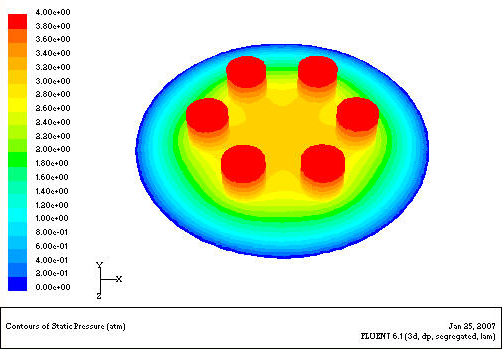
\includegraphics[width=0.5\linewidth]{figures/1.png} %{}内为图片的路径
\figcaptioncneng{局部多孔质圆柱塞半径不同时轴承的压力分布云图} % 图片的中文标题
                {Pressure contour of bearing with partial porous plunger different radiuses} % 图片的英文标题
\label{fig:system} % 正文中通过\ref{fig:system} 引用该图片
\end{figure*}

从图~\ref{fig:bearing-pressure}可知，由于节流半径不同，导致节流效果产生很大的不同，其中，半径小的节流效果明显，图~\subref{subfig:bearing-15}对应的压力变化最明显，而图~\subref{subfig:bearing-45}的变化非常小，这导致了气膜内的压力分布产生了很大的不同。从而使承载能力随着半径的增加而得到很大的提高。从图~\ref{fig:bearing-pressure}可知，由于节流半径不同，导致节流效果产生很大的不同，其中，半径小的节流效果明显，图~\subref{subfig:bearing-15}对应的压力变化最明显，而图~\subref{subfig:bearing-45}的变化非常小，这导致了气膜内的压力分布产生了很大的不同。从而使承载能力随着半径的增加而得到很大的提高。从图~\ref{fig:bearing-pressure}可知，由于节流半径不同，导致节流效果产生很大的不同，其中，半径小的节流效果明显，图~\subref{subfig:bearing-15}对应的压力变化最明显，而图~\subref{subfig:bearing-45}的变化非常小，这导致了气膜内的压力分布产生了很大的不同。从而使承载能力随着半径的增加而得到很大的提高。从图~\ref{fig:bearing-pressure}可知，由于节流半径不同，导致节流效果产生很大的不同，其中，半径小的节流效果明显，图~\subref{subfig:bearing-15}对应的压力变化最明显，而图~\subref{subfig:bearing-45}的变化非常小，这导致了气膜内的压力分布产生了很大的不同。从而使承载能力随着半径的增加而得到很大的提高。

从图~\ref{fig:bearing-pressure}可知，由于节流半径不同，导致节流效果产生很大的不同，其中，半径小的节流效果明显，图~\subref{subfig:bearing-15}对应的压力变化最明显，而图~\subref{subfig:bearing-45}的变化非常小，这导致了气膜内的压力分布产生了很大的不同。从而使承载能力随着半径的增加而得到很大的提高。

\begin{figure}[h]
  \centering
  % 第一行：两个子图并排，[b]底部对齐，[t]顶部对齐
  \begin{subfigure}[b]{0.48\textwidth}
    \centering
    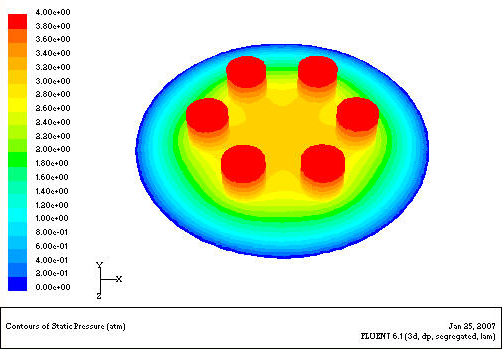
\includegraphics[width=\textwidth]{figures/1.png} %{}内为图片的路径
    \subfigcaptioncneng{$R_3$=1.5mm 时轴承的压力分布云图。} % 子图的中文标题
                      {Pressure contour of bearing when $R_3$=1.5mm。} % 子图的英文标题
    \label{subfig:bearing-15} % 子图标签
  \end{subfigure}
  \hfill
  \begin{subfigure}[b]{0.48\textwidth}
    \centering
    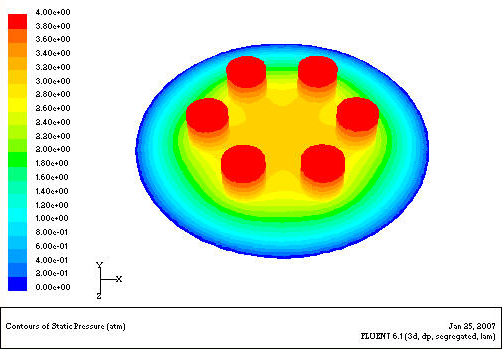
\includegraphics[width=\textwidth]{figures/1.png}
    \subfigcaptioncneng{$R_3$=2.5mm 时轴承的压力分布云图。}
                      {Pressure contour of bearing when $R_3$=2.5mm。}
    \label{subfig:bearing-25}
  \end{subfigure}
  \vspace{1em} % 两行之间的间距
  
  % 第二行：两个子图并排
  \begin{subfigure}[b]{0.48\textwidth}
    \centering
    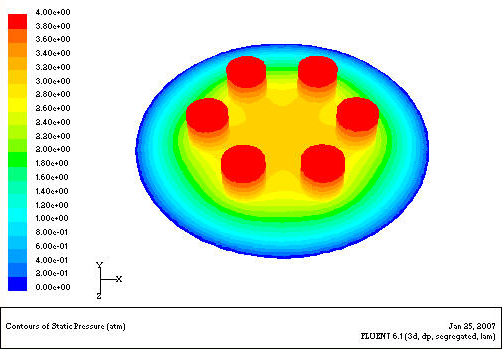
\includegraphics[width=\textwidth]{figures/1.png}
    \subfigcaptioncneng{$R_3$=3.5mm 时轴承的压力分布云图。}%
                      {Pressure contour of bearing when $R_3$=3.5mm。}
    \label{subfig:bearing-35}
  \end{subfigure}
  \hfill
  \begin{subfigure}[b]{0.48\textwidth}
    \centering
    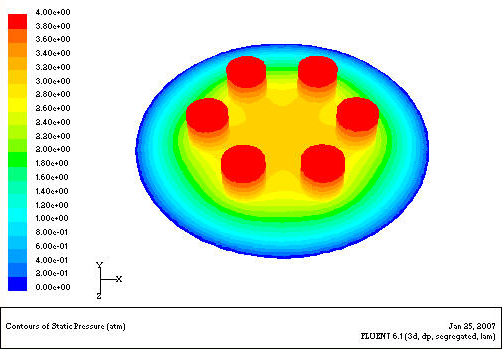
\includegraphics[width=\textwidth]{figures/1.png}
    \subfigcaptioncneng{$R_3$=4.5mm 时轴承的压力分布云图。}%
                      {Pressure contour of bearing when $R_3$=4.5mm。}
    \label{subfig:bearing-45}
  \end{subfigure}
  
  % 主图标题
  \figcaptioncneng{局部多孔质圆柱塞半径不同时轴承的压力分布云图。} % 主图的中文标题
                  {Pressure contour of bearing with partial porous plunger different radiuses。} % 主图的英文标题
  \label{fig:bearing-pressure} % 主图的标签
\end{figure}

从图~\ref{fig:bearing-pressure}可知，由于节流半径不同，导致节流效果产生很大的不同，其中，半径小的节流效果明显，图~\subref{subfig:bearing-15}对应的压力变化最明显，而图~\subref{subfig:bearing-45}的变化非常小，这导致了气膜内的压力分布产生了很大的不同。
  \chapter{局部多孔质静压轴承的实验研究}
\echapter{Experimental Study on Local Porous Hydrostatic Bearings}

学位论文的结论作为论文正文的最后一章单独排写。
结论是对整个论文主要成果的总结。在结论中应明确指出本研究内容的创造性成果或创新点理论（含新见解、新观点），并指出今后进一步在本研究方向进行研究工作的展望与设想，不要将结论写成论文的摘要。结论内容一般在2000字以内。

\textbf{表格单条注释使用示例：}
\begin{table}[htbp]
%----------------------中文标题
\bilingualtablecaption{1号试样渗透率测试数据（温度：T=16℃ 高度：H=5.31mm）} % 表格中文标题
{Data of measured permeability of sample 1 (Temperature: T=16℃ Height: H=5.31mm)} % 表格英文标题
\label{notation} % 通过\ref{notation}实现对该表的引用
% 可以通过修改C{}大括号内的数值设置各列宽度，所有大括号里的数字加起来必须正好等于1。
\begin{tabularx}{\textwidth}{ C{0.4} C{0.6}}
    \toprule[1.5pt]
        %----------------------表头
        Notation & Description   \\  
        %----------------------
    \midrule[1pt]
    %---------------------- 表格内容
        $P_{t}^L$ & Users' energy consumption \\ 
        $P_t^{gen}$ & The power of generator\\
        $P_t^{PV}$ & PV power \\ 
        $P_t^{WT}$ & WT power  \\
        $P_t^{sell}$ & The power sold to main gird \\ 
        $P_t^{buy}$ & The power bought from main grid \\
    %----------------------
    \bottomrule[1.5pt]
\end{tabularx}
\\[4pt]  % 新增
\parbox{\textwidth}{\footnotesize 注：此处填写你的注释内容。} % 新增
\end{table}


\textbf{表格多条注释使用示例：}
\begin{table}[htbp]
%----------------------中文标题
\bilingualtablecaption{1号试样渗透率测试数据（温度：T=16℃ 高度：H=5.31mm）} % 表格中文标题
{Data of measured permeability of sample 1 (Temperature: T=16℃ Height: H=5.31mm)} % 表格英文标题
\label{notation} 
\begin{threeparttable}  % 新增
\begin{tabularx}{\textwidth}{ C{0.4} C{0.6}}
    \toprule[1.5pt]
        %----------------------表头
        Notation & Description   \\  
        %----------------------
    \midrule[1pt]
    %---------------------- 表格内容
        $P_{t}^L$ & Users' energy consumption \\ 
        $P_t^{gen}$ & The power of generator\\
        $P_t^{PV}$ & PV power \\ 
        $P_t^{WT}$ & WT power  \\
        $P_t^{sell}$ & The power sold to main gird \tnote{2}\\ 
        $P_t^{buy}$ & The power bought from main grid \tnote{1}\\
    %----------------------
    \bottomrule[1.5pt]
\end{tabularx}
\begin{tablenotes}  % 新增
    \footnotesize  % 新增
    \item[1] 这里是对该项的具体注释说明。 % 新增
    \item[2] 这里是对该项的具体注释说明。 % 新增
\end{tablenotes}   % 新增
\end{threeparttable}  % 新增
\end{table}


\textbf{跨页长表格单条注释使用示例：}
% 可以通过修改C{}大括号内的数值设置各列宽度，所有大括号里的数字加起来必须正好等于1。
\begin{longtable}{C{0.15} C{0.15} C{0.25} C{0.15} C{0.15} C{0.15}}
%----------------------中文标题
\bilingualtablecaption{1号试样渗透率测试数据（温度：T=16℃ 高度：H=5.31mm）} % 表格中文标题
{Data of measured permeability of sample 1 (Temperature: T=16℃ Height: H=5.31mm)} % 表格英文标题
\label{tab:permeability} \\ % 通过\ref{tab:permeability}实现对该表的引用

%----------------------表头
\toprule[1.5pt]
供气压力 & 流量测量 & 流量修正值 & 压力差 & $\lg \Delta P$ & $\lg M$ \\ 
$P_g$ (MPa) & $M'$ (m$^3$/h) & $M$ ($\times10^{-4}$ m$^3$/s) & $\Delta P$ (Pa) & & \\  % 表头信息
\midrule[1pt]
\endfirsthead

%----------------------续表表头
\multicolumn{6}{r}{{\thenexttable}} \\ % 续表标记
\toprule[1.5pt]
供气压力 & 流量测量 & 流量修正值 & 压力差 & $\lg \Delta P$ & $\lg M$ \\ 
$P_g$ (MPa) & $M'$ (m$^3$/h) & $M$ ($\times10^{-4}$ m$^3$/s) & $\Delta P$ (Pa) & & \\ % 续表的表头信息
\midrule[1pt]
\endhead

%----------------------非最后一页页尾
\midrule[1.5pt]
% \multicolumn{6}{r}{\zihao{5} 接下表} \\
\endfoot

\bottomrule[1.5pt]    % 新增
\multicolumn{6}{l}{\parbox{\linewidth}{\footnotesize   % 新增
注：此处填写你的表格注释内容。}}   % 新增
\endlastfoot   % 新增

%---------------------- 表格内容
0.35 & 0.136 & 0.21753 & 246900 & 5.39252 & -4.66248\tnote{2} \\  
0.40 & 0.171 & 0.25485 & 296900 & 5.47261 & -4.59372 \\
0.35 & 0.136 & 0.21753 & 246900 & 5.39252 & -4.66248 \\
0.40 & 0.171 & 0.25485 & 296900 & 5.47261 & -4.59372 \\
0.35 & 0.136 & 0.21753 & 246900 & 5.39252 & -4.66248 \\
0.40 & 0.171 & 0.25485 & 296900 & 5.47261 & -4.59372 \\
0.35 & 0.136 & 0.21753 & 246900 & 5.39252 & -4.66248 \\
0.40 & 0.171 & 0.25485 & 296900 & 5.47261 & -4.59372 \\
0.35 & 0.136 & 0.21753 & 246900 & 5.39252 & -4.66248 \\
0.40 & 0.171 & 0.25485 & 296900 & 5.47261 & -4.59372 \\
0.45 & 0.202 & 0.28467 & 346900 & 5.54020 & —— 
\end{longtable}


\textbf{跨页长表格多条注释使用示例：}

\begin{ThreePartTable}   % 新增
\begin{TableNotes}   % 新增
    \footnotesize  % 新增
    \item[1] 这里是注释1的内容。   % 新增
    \item[2] 这里是注释2的内容。   % 新增
\end{TableNotes}   % 新增
\begin{longtable}{C{0.15} C{0.15} C{0.25} C{0.15} C{0.15} C{0.15}}
%----------------------中文标题
\bilingualtablecaption{1号试样渗透率测试数据（温度：T=16℃ 高度：H=5.31mm）} % 表格中文标题
{Data of measured permeability of sample 1 (Temperature: T=16℃ Height: H=5.31mm)} % 表格英文标题
\label{tab:permeability} \\ % 通过\ref{tab:permeability}实现对该表的引用

%----------------------表头
\toprule[1.5pt]
供气压力 & 流量测量 & 流量修正值 & 压力差 & $\lg \Delta P$ & $\lg M$ \\ 
$P_g$ (MPa) & $M'$ (m$^3$/h) & $M$ ($\times10^{-4}$ m$^3$/s) & $\Delta P$ (Pa) & & \\  % 表头信息
\midrule[1pt]
\endfirsthead

%----------------------续表表头
\multicolumn{6}{r}{{\thenexttable}} \\ % 续表标记
\toprule[1.5pt]
供气压力 & 流量测量 & 流量修正值 & 压力差 & $\lg \Delta P$ & $\lg M$ \\ 
$P_g$ (MPa) & $M'$ (m$^3$/h) & $M$ ($\times10^{-4}$ m$^3$/s) & $\Delta P$ (Pa) & & \\ % 续表的表头信息
\midrule[1pt]
\endhead

%----------------------非最后一页页尾
\midrule[1.5pt]
% \multicolumn{6}{r}{\zihao{5} 接下表} \\
\endfoot

\bottomrule[1.5pt]   % 新增
\insertTableNotes    % 新增
\endlastfoot   % 新增

%---------------------- 表格内容
0.35 & 0.136 & 0.21753 & 246900 & 5.39252 & -4.66248\tnote{1} \\  
0.40 & 0.171 & 0.25485 & 296900 & 5.47261 & -4.59372 \tnote{2}\\
0.35 & 0.136 & 0.21753 & 246900 & 5.39252 & -4.66248 \\
0.40 & 0.171 & 0.25485 & 296900 & 5.47261 & -4.59372 \\
0.35 & 0.136 & 0.21753 & 246900 & 5.39252 & -4.66248 \\
0.40 & 0.171 & 0.25485 & 296900 & 5.47261 & -4.59372 \\
0.35 & 0.136 & 0.21753 & 246900 & 5.39252 & -4.66248 \\
0.40 & 0.171 & 0.25485 & 296900 & 5.47261 & -4.59372 \\
0.35 & 0.136 & 0.21753 & 246900 & 5.39252 & -4.66248 \\
0.40 & 0.171 & 0.25485 & 296900 & 5.47261 & -4.59372 \\
0.45 & 0.202 & 0.28467 & 346900 & 5.54020 & —— 
\end{longtable}
\end{ThreePartTable}    % 新增


  \chapter{结论与展望}
\echapter{Conclusions and prospects}

学位论文的结论作为论文正文的最后一章单独排写~\upcite{chen2001hao}。
~\upcite{clerc2010discrete, liu1979, maoxia, xia2002analysis, 1025090578.nh}，~\upcite{xia2002analysis, 1025090578.nh, xxx2023}, ~\upcite{award2007,gbt16159,maoxia2000,feng1997,wang1998}

结论是对整个论文主要成果的总结。在结论中应明确指出本研究内容的创造性成果或创新点理论（含新见解、新观点），并指出今后进一步在本研究方向进行研究工作的展望与设想，不要将结论写成论文的摘要。结论内容一般在2000字以内。学位论文的结论作为论文正文的最后一章单独排


  

%%----------- 结尾部分 ----------- %%
  \chapterstar{参考文献}
\echapterstar{Reference}
\bibliographystyle{tools/gbt7714-numerical}
\bibliography{others/reference}       % 参考文献
  %  附录部分使用代码
  \appendix
  \chapter{附录标题示例}
\echapter{Example of Appendix Title}

附录作为主体部分的补充，并不是必须的。

下列内容可以作为附录编于论文后

——为了整篇论文材料的完整，但编入正文又有损于编排的条理性和逻辑性，这一材料包括比正文更为详尽的信息、研究方法和技术更深入的叙述，对了解正文内容有用的补充信息等；

——由于篇幅过大或取材于复制品而不便于编入正文的材料；

——不便于编入正文的罕见珍贵资料；

——对一般读者并非必要阅读，但对本专业同行有参考价值的资料；

——某些重要的原始数据、数学推导、结构图、统计表、计算机打印输出件等。 
  \stopappendix
  
  
\chapterstar{攻读博士学位期间发表的论文及其它成果}
\echapterstar{Papers published in the period of Ph.D. education}

\boldparafirst{（一）发表的学术论文} 

\begin{achievementlist}
\item[ {[1]} ]
xxx，xxx．局部多孔质气体静压轴向轴承静态特性的数值求解[J]．
摩擦学学报，2007，38(12)：68--72．
（EI收录号：20071510544816）
\item[ {[2]} ]
xxx，xxx．．
\end{achievementlist}

\boldpara{（二）申请及已获得的专利（无专利时此项不必列出）}

\begin{achievementlist}
\item[ {[1]} ]
xxx，xxx. 一种温热外敷药制备方案：中国，88105607.3［P］. 1989-07-26．
\end{achievementlist}

\boldpara{（三）获得的科技奖励（无获奖时此项不必列出）}
\begin{achievementlist}
\item[ {[1]} ]
xxx，xxx. xx静载下预应力混凝土房屋结构设计统一理论. 黑龙江省科学技术二等奖, 2007.
\end{achievementlist}

注：如已发表的学术论文被EI或SCI收录，请标明收录号及SCI论文的影响因子；对已接收但尚未发表出来的学术论文，请注明是否EI或SCI刊源。    % 攻读博士学位期间发表的论文及其他成果
  \chapterstar{攻读博士学位期间参加的科研工作}
\echapterstar{Research Work in the period of Ph.D. education}

\begin{achievementlist}
\item[ {[1]} ]

\item[ {[2]} ]

\end{achievementlist}
   % 攻读博士学位期间参加的科研工作
  \chapterstar[致谢]{致~~~~ 谢}
\echapterstar{Acknowledgements}

衷心感谢导师xxx教授对本人的精心指导。他的言传身教将使我终生受益。
感谢xxx教授，以及实验室全体老师和同窗们的热情帮助和支持！

本课题承蒙xxx基金资助，特此致谢。

最后，感谢你一直以来的努力，祝你博士毕业快乐！！！！    % 致谢
  \chapterstar{作者简介}
\echapterstar{Resume}

xxxx年xx月xx日出于xxxx。

xxxx年xx月考入xx大学xx院（系）xx专业，xxxx年xx月本科毕业并获得xx学学士学位。

xxxx年xx月——xxxx年xx月在xx大学xx院（系）xx学科学习并获得xx学硕士学位。

xxxx年xx月——xxxx年xx月在xx大学xx院（系）xx学科学习并获得xx学博士学位。

获奖情况：如获三好学生、优秀团干部、x奖学金等（不含科研学术获奖）。

工作经历：  % 作者简介
  

\end{document}